\documentclass[10pt]{article}
\usepackage[framemethod=TikZ]{mdframed}
\usepackage{amsthm}
\usepackage[landscape]{geometry}
\usepackage{multicol}
\usepackage{tikz}
\usepackage{pgfplots}
\usepackage{xcolor}
\usepackage{amsmath}
\usepackage[T1]{fontenc}
\usepackage{utopia}
\usepackage{changepage}
\usepackage{amssymb}
\usepackage{fancyhdr}
\usepackage[many]{tcolorbox}
\usepackage{moresize}
\usepackage{fullpage}
\usepackage{mathpazo}
\usepackage{tikz-3dplot}
\usepackage{cancel}
\tdplotsetmaincoords{70}{165}
\pgfplotsset{compat=1.18}
\usepackage{enumitem}
\usepackage{tabularray}
\usepackage{mathtools}

\UseTblrLibrary{diagbox}

\usetikzlibrary{
    shadings, calc, patterns, angles, quotes, arrows.meta, 
    decorations.pathmorphing, decorations.pathreplacing, 
    fadings, 3d, perspective, backgrounds, intersections, 
    decorations.markings, bending, positioning, 							spy,shapes.geometric,shadows,shapes.symbols, fadings, matrix, fit
}

\usepgfplotslibrary{
    groupplots, external, colormaps, patchplots, fillbetween
}


\setlength{\baselineskip}{1.2em}
\setlength{\parskip}{-0.75em}
\setlist{topsep=0pt, leftmargin=1cm, noitemsep}

% Reds (r)
\definecolor{r1}{RGB}{255, 191, 191}    % Light coral
\definecolor{r2}{RGB}{255, 191, 223}    % Light pink
\definecolor{r3}{RGB}{255, 207, 207}    % Light rose

% Blues (b)
\definecolor{b1}{RGB}{191, 223, 255}    % Light blue
\definecolor{b2}{RGB}{191, 239, 255}    % Light sky
\definecolor{b3}{RGB}{191, 255, 255}    % Light cyan

% Greens (g)
\definecolor{g1}{RGB}{191, 255, 191}    % Light green
\definecolor{g2}{RGB}{191, 255, 223}    % Light mint
\definecolor{g3}{RGB}{207, 255, 207}    % Light sage

% Oranges (o)
\definecolor{o1}{RGB}{255, 223, 191}    % Light peach
\definecolor{o2}{RGB}{255, 239, 191}    % Light cream
\definecolor{o3}{RGB}{255, 231, 191}    % Light buff

% Violets (v)
\definecolor{v1}{RGB}{223, 191, 255}    % Light purple
\definecolor{v2}{RGB}{239, 191, 255}    % Light lilac
\definecolor{v3}{RGB}{231, 191, 255}    % Light lavender

% Yellows (y)
\definecolor{y1}{RGB}{255, 255, 191}    % Light yellow
\definecolor{y2}{RGB}{255, 247, 191}    % Light cream yellow
\definecolor{y3}{RGB}{255, 239, 191}    % Light warm cream

\definecolor{w}{HTML}{eeeeee}
\definecolor{g}{HTML}{444444}
\definecolor{b}{HTML}{222222}
\definecolor{lightgrey}{HTML}{cccccc}
\definecolor{firebrick}{RGB}{178, 34, 34}
\definecolor{myg}{RGB}{3, 252, 177}

\geometry{
    letterpaper,
    left=0.25in,
    right=0.25in,
    top=0.15in,
    bottom=0.25in
}

\newcommand{\hr}{\centerline{\rule{3.5in}{1pt}}}

\newcommand{\nc}[2][b]{%
\tikz \draw [draw=#1,ultra thick]
    ($(current page.center)-(0.495\linewidth,0)$) -- 
    ($(current page.center)+(0.495\linewidth,0)$)
    node [midway, fill=b] {\ssmall\textbf{\uppercase{#2}}};
}
\newcommand{\nsc}[2][b]{%
\tikz \draw [draw=#1,ultra thick, dashed]
    ($(current page.center)-(0.495\linewidth,0)$) -- 
    ($(current page.center)+(0.495\linewidth,0)$)
    node [midway, fill=b] {\ssmall\textbf{\uppercase{#2}}};
}

\newtcolorbox{conceptbox}[2][]{
	breakable,
	vfill before first=false,
	segmentation at break=false,
	size=fbox,
	colback=b,
	title=\scriptsize\textbf{\MakeUppercase{#2}},
	left=2pt,
	right=2pt,
	top=3pt,
	bottom=1pt,
	boxrule=1pt,
	coltitle=b,
	colupper=w,
	pad at break=5pt,
	toprule at break=4pt,
	bottomrule at break=0.75pt,
	colframe=#1,
	enlargepage=12in, 
	before upper*={\setlength{\baselineskip}{0.75em}\setlength{\parskip}{0em}}
}

\newtcolorbox{quotebox}[1][blue!50!green]{
	arc=0mm,
	interior engine=path,
	interior style={top color=#1, bottom color=#1!20!white},
	colframe=b
}

\newcommand{\drawf}[2]{
	\draw[ultra thick, -stealth] (#1-1, 0) -- (#1+9, 0) node[right] {$x$};
	\draw[ultra thick, -stealth] (0, #2-4) -- (0, #2+4) node[above] {$y$};
	\draw[thick, draw=b1] 
	(#1, #2) .. controls +(1, 3.5) and +(-1, 2.5) .. +(2, 1.5)
	.. controls +(0.65, -1.5) .. +(2.9, 1) 
	.. controls +(0.4, 2) .. +(6, -3)
	.. controls +(0.4, -1) .. +(8, 0);
	
	\draw[dashed, draw=o1] (#1, #2) -- +(8, 0);	
	
	\filldraw[fill=firebrick] (#1, #2) circle(3pt);
	\node[outer sep=2pt, above left, rotate=30] at (#1, #2) {$(a, f(a))$};
	\node[outer sep=2pt, below] at (#1, 0) {$a$};
	\draw[draw=o1, dashed] (#1, 0) -- (#1, #2);
	
	\filldraw[fill=firebrick] ($(#1, #2) + (8, 0)$) circle(3pt);
	\node[outer sep=3pt, above right, rotate=-30] at ($(#1, #2) + (8, 0)$) {$(b, f(b))$};
	\node[outer sep=2pt, below] at ($(#1, 0) + (8, 0)$) {$b$};
	\draw[draw=o1, dashed] ($(#1, 0) + (8, 0)$) -- ($(#1, #2) + (8, 0)$);
	
	\filldraw[draw=o1, fill=firebrick] ($(#1, #2) + (1.12, 3.07)$) circle (2pt);
	\draw[draw=blue!20!red, thick] (#1 - 1.5, #2 + 3.07) -- (#1 + 4.7, #2 + 3.07);
	\node[outer sep=2pt, above] at ($(#1, #2) + (1.12, 3.07)$) {$(c, f(c))$};
	\node[outer sep=2pt, below] at (#1 + 1.12, 0) {$c$};
	\draw[draw=o1, dashed] (#1 + 1.12, 0) -- (#1 + 1.12, #2 + 3.07);
	
	\node[] (val) at (0, #2) {};
	\filldraw[draw=o1, fill=firebrick] (0, #2) circle (2pt);
	\node[draw=v2, below left, outer sep=1pt, rotate=-20, shape=ellipse, double=b, double distance=2pt] (vals) at ($(0, #2) + (4, 3)$)  {$f(a) = f(b)$};
	\draw[->, draw=v1, >={Stealth[round]},semithick] (val.east) .. controls +(right:1cm) and +(down:1cm) .. (vals.south);
	
	\node[] (cp) at ($(#1, #2) + (1.12, 3.07)$) {};
	\node[scale=0.7, draw=v2, below left, outer sep=1pt, rotate=-20, shape=ellipse, double=b, double distance=2pt] (cps) at ($(#1, #2) + (1.12, 3.07) + (-1.5, -1.5)$)  {$f'(c) = 0$};
	\draw[->, draw=v1, >={Stealth[round]},semithick] (cp.west) .. controls +(225:1cm) and +(up:1cm) .. (cps.north);
}

\newcommand{\drawfspy}[2]{
	\draw[draw=w, ultra thick, -stealth] (-4-1, 0) -- (-4+9, 0) node[text=w, right] {$x$};
	\draw[draw=w, ultra thick, -stealth] (0, 2.5-4) -- (0, 2.5+4) node[text=w, above] {$y$};
	\draw[thick, draw=b1] 
	(-4, 2.5) .. controls +(1, 3.5) and +(-1, 2.5) .. +(2, 1.5)
	.. controls +(0.65, -1.5) .. +(2.9, 1) 
	.. controls +(0.4, 2) .. +(6, -3)
	.. controls +(0.4, -1) .. +(8, 0);
	
	\draw[dashed, draw=o1] (-4, 2.5) -- +(8, 0);	
	
	\filldraw[fill=firebrick] (-4, 2.5) circle(3pt);
	\node[text=w, outer sep=2pt, above left, rotate=30] at (-4, 2.5) {$(a, f(a))$};
	\node[text=w, outer sep=2pt, below] at (-4, 0) {$a$};
	\draw[draw=o1, dashed] (-4, 0) -- (-4, 2.5);
	
	\filldraw[fill=firebrick] ($(-4, 2.5) + (8, 0)$) circle(3pt);
	\node[text=w, outer sep=3pt, above right, rotate=-30] at ($(-4, 2.5) + (8, 0)$) {$(b, f(b))$};
	\node[text=w, outer sep=2pt, below] at ($(-4, 0) + (8, 0)$) {$b$};
	\draw[draw=o1, dashed] ($(-4, 0) + (8, 0)$) -- ($(-4, 2.5) + (8, 0)$);

	\filldraw[draw=o1, fill=firebrick] (0, 2.5) circle (2pt);
	\filldraw[draw=o1, fill=firebrick] (1.77, 0) circle (2pt);
	\filldraw[draw=o1, fill=firebrick] (2.98, 0) circle (2pt);
	
}

\begin{document}
\ssmall
\pagecolor{b}
\fontfamily{put}

\begin{minipage}{\textwidth} %title
	\tikz{
		\node[anchor=west, fill=o1, outer sep=1mm] (A) at ($(current page.center)-(0.495\linewidth,0)$) {\textbf{Adam Andrei}};
		\node[anchor=east, fill=o1, outer sep=1mm] (B) at ($(current page.center)+(0.5\linewidth,0)$) {\textbf{27.12.2024}};
		\node[fill=o1, outer sep=1mm, align=center] (C) at ($(current page.center)$) {\huge\textbf{\uppercase{Teorema lui Rolle.}} \\ \huge\textbf{\uppercase{Șirul lui Rolle.}}};
		
		\draw [draw=o1,ultra thick] (A) -- (C) -- (B);
	}
\end{minipage}


\begin{multicols*}{3}
	\begin{conceptbox}[v3]{Teorema lui Rolle}
		\nc[o1]{EnunȚ}
		\begin{quotebox}
			\quad Fie o funcție $f: \left[a, b\right]\to\mathbb{R}$ cu următoarele proprietăți:
			\begin{itemize}
				\item $f$ este continuă pe $\left[a, b\right]$
				\item $f$ este derivabilă pe $\left(a, b\right)$
				\item $f(a) = f(b)$
			\end{itemize}
		atunci există $c\in \left(a, b\right)$ astfel încât \textcolor{firebrick}{f'(c) = 0}.			 
		\end{quotebox}
		\bigskip
		\nsc[o1]{DemonstraȚie}
		\begin{center}
			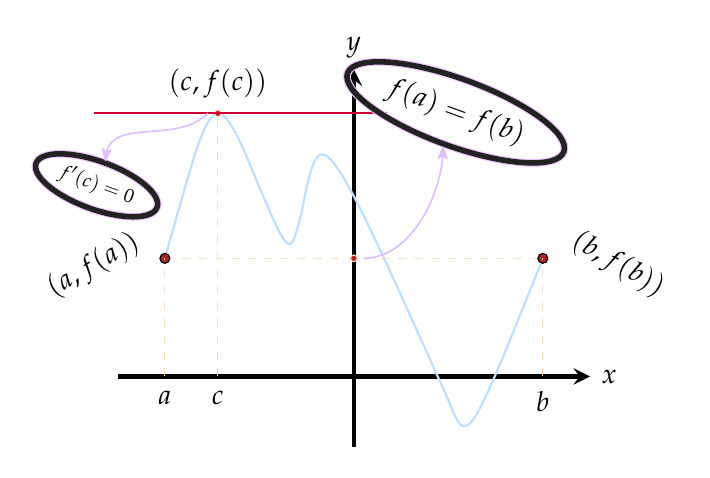
\begin{tikzpicture}[scale=0.6]
				\drawf{-4}{2.5}
			\end{tikzpicture}
		\end{center}
		\quad Dacă $f$ e o funcție constantă $\Rightarrow$ concluzia e evidentă.\\
		
		\quad Presupunem în continuare că $f$ nu este o funcție constantă. Cum $f$ este o funcție continuă pe un interval închis, atunci conform \textit{teoremei lui Weierstrass} știm că $f$ este mărginită și își atinge marginile. Cu alte cuvinnte, $f$ admite punct de minim și punct de maxim.\\
		
		\quad Fie $m, M \in \left[a, b\right]$ punctul de \textit{minim}, respectiv de \textit{maxim} a funcției $f$ și fie $v:= f(a)=f(b)$. \\
		
\quad $f$ nu este constantă $\Rightarrow m \neq M$ și $f(m) \neq f(M) \Rightarrow f(m) \neq v$ sau $f(M) \neq v \Rightarrow \\ \Rightarrow m \notin \left\lbrace a, b \right\rbrace$  sau $M \notin \left\lbrace a, b \right\rbrace \Rightarrow m \in \left(a, b\right)$ sau $M \in \left(a, b\right) \Rightarrow f$ are un punct de extrem în intervalul deschis $\left(a, b\right)$.\\

\quad Dar din \textit{teorema lui Fermat} știm că punctele de extrem dintr-un interval deschis ale unei funcții derivabile se găsesc printre punctele critice ale funcției (a.k.a punctele $x$ cu proprietatea că $f'(x) = 0$), deci fie $f'(m) = 0$ fie $f'(M) = 0$.  \\

\quad În concluzie există $c \in \left(a, b\right)$ (cel puțin unul dintre $m$ și $M$) astfel încât $f'(c) = 0$. 
	\end{conceptbox}
	\begin{conceptbox}[r1]{Caz de interes}
	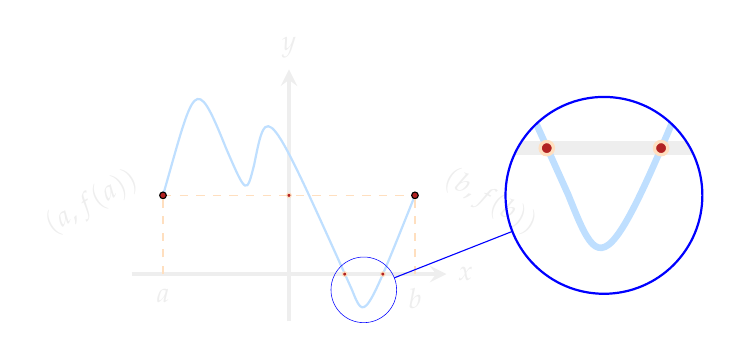
\begin{tikzpicture}[scale=0.4,
	 spy using outlines={circle, magnification=3, size=2.5cm, connect spies}
]
				\drawfspy{-4}{2.5}
				\spy[blue] on (0.95, -0.2) in node at (10, 2.5);
			\end{tikzpicture}
			
\quad	Un caz particular în care se poate aplica \textit{teorema lui Rolle} este asupra restricției unei funcții la intervalul cuprins între două \textit{zerouri} (\textit{rădăcini ale funcției}).\\
	
	\quad Fie $x_1 \neq x_2 \in \left[a, b\right]$ două rădăcini ale funcției $f \Rightarrow f(x_1) = f(x_2) = 0$. Aplicând \textit{teorema lui Rolle} restricției funcției $f$ la intervalul $\left[x_1, x_2\right]$ obținem: \[ \left(\exists \right) x_0 \in \left(x_1, x_2\right) \text{ a.î. } f'(x_0) = 0\] 
			\begin{quotebox}[green!20!red]
			\quad Deci între două rădăcini ale unei funcții există cel puțin o rădăcină a derivatei.
			\end{quotebox}
			\nsc[o1]{ConsecinȚĂ}
			
			\quad Fie acum $x_1'<x_2'\in\left(a, b\right)$ două rădăcini \textit{\textbf{\textcolor{firebrick}{consecutive}}} ale derivatei $f'$. Presupunem prin absurd că există \textit{\textbf{\textcolor{firebrick}{două rădăcini distincte}}} ale funcției $f$ în intervalul $\left[x_1', x_2'\right]$. Dar atunci există un $x_0 \in \left(x_1', x_2'\right)$ astfel încât $f'(x_0) = 0$ (deoarece între două rădăcini ale funcției există o rădăcină a derivatei), ceea ce contrazice faptul că $x_1'$ și $x_2'$ sunt rădăcini consecutive ale derivatei. Deci:
			\begin{quotebox}[yellow!70!black]
				\quad Între \textit{\textbf{\textcolor{firebrick}{două rădăcini consecutive}}} ale derivatei $f'$ nu pot să existe două rădăcini distincte ale funcției $f$. Prin urmare avem:
				\begin{quotebox}[v1]
				\quad	\textit{\textbf{\textcolor{firebrick}{Între două rădăcini consecutive ale derivatei există cel mult o rădăcină a funcției.}}}
				\end{quotebox}
			\end{quotebox}
	\end{conceptbox}
	\begin{conceptbox}[brown]{INTERPRETĂRI}
		\nc[o1]{INTERPRETARE GEOMETRICĂ}
		
		\quad Fie $f:\left[a, b\right]\to\mathbb{R}$ o funcție care respectă cerințele din \textit{teorema lui Rolle}, atunci există un punct $c\in\left(a, b\right)$ în care tangenta la graficul funcției are \textit{\textcolor{firebrick}{panta 0}} (adică este paralelă cu axa \textit{Ox}).
		
		
		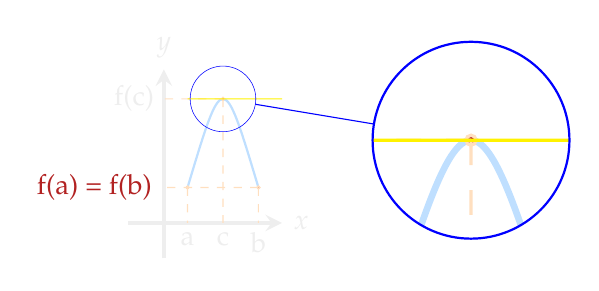
\begin{tikzpicture}[scale=0.3,
	 spy using outlines={circle, magnification=3, size=2.5cm, connect spies}
]
			\draw[draw=w, ultra thick, -stealth] (-1.5, 0) -- (5, 0) node[text=w, right] {$x$};
			\draw[draw=w, ultra thick, -stealth] (0, -1.5) -- (0, 6.5) node[text=w, above] {$y$};
						
			\coordinate (A) at (1, 1.5);
			\coordinate (B) at (4, 1.5);
			\coordinate (C) at ($(A)!0.5!(B) + (0, 3.75)$);
			
			\coordinate (Bezier) at ($(A)!0.5!(B) + (0, 5)$);	
			
			\draw[thick, draw=b1] (A) .. controls (Bezier) .. (B);
			
			\filldraw[draw=o1, fill=firebrick] (A) circle (2pt);
			\filldraw[draw=o1, fill=firebrick] (B) circle (2pt);
			\filldraw[draw=o1, fill=firebrick] (C) circle (2pt);
			
			\coordinate (Ax) at (A |- 0, 0);
			\coordinate (Ay) at (A -| 0, 0);
			
			\coordinate (Bx) at (B |- 0, 0);
			\coordinate (By) at (B -| 0, 0);
			
			\coordinate (Cx) at (C |- 0, 0);
			\coordinate (Cy) at (C -| 0, 0);			
			
			\draw[dashed, draw=o1] (A) -- (Ax)	;
%			\draw[dashed, draw=o1] (A) -- (Ay)	;
			
			\draw[dashed, draw=o1] (B) -- (Bx)	;
			\draw[dashed, draw=o1] (B) -- (By)	;

			\draw[dashed, draw=o1] (C) -- (Cx)	;
			\draw[dashed, draw=o1] (C) -- (Cy)	;
			
			
			\node[below, text=w] at (Ax) {a};
			\node[below, text=w] at (Bx) {b};
			\node[below, text=w] at (Cx) {c};
			\node[left, outer sep=1pt] at (Ay) {\textcolor{firebrick}{f(a) = f(b)}};
			\node[left, text=w] at (Cy) {f(c)};	
			
			\draw[draw=yellow] ($(Cy)!0.4!(C)$) -- ($(Cy)!2!(C)$);
				
			\spy[blue] on (C) in node at (13, 3.5);
			
		\end{tikzpicture}
		
		\nc[o1]{INTERPRETARE FIZICĂ}
		
		\quad Considerăm un drum fără bucle (nu se poate ajunge în același loc mergând în față) și o particulă (om, mașină, etc.) care parcurge drumul. Fie acum funcția $f$ care are ca argument timpul $t$ scurs de la plecare și ca rezultat $f(t)$ - distanța dintre punctul de plecare și punctul curent. În acest context, derivata $f'(t) =\displaystyle \lim_{\Delta t \to 0}\dfrac{\Delta f(t)}{\Delta t}$ reprezintă \textit{\textcolor{b1}{viteza}} particulei.

		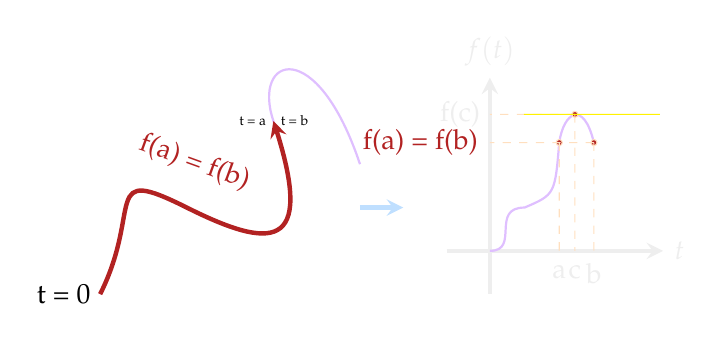
\begin{tikzpicture}[scale=0.55]
			\coordinate (c1) at (-5, -1);
			\coordinate (c2) at (-3, 1);
			\coordinate (c3) at (-1, 3);
			\coordinate (c4) at (1, 2);
			
			\coordinate (b1) at	($(c1) + (1, 2)$);
			
			\coordinate (b21) at ($(c2) + (-2, 1)$);
			\coordinate (b22) at ($(b21)!2!(c2)$);
			
			\coordinate (b31) at ($(c3) + (1, -3)$);
			\coordinate (b32) at ($(b31)!1.5!(c3)$);
			
			\coordinate (b41) at ($(c4) + (-1, 3)$);
			
			\draw[draw=v1, thick] (c1) .. controls (b1) and (b21) .. (c2)
				.. controls (b22) and (b31) .. (c3)
				.. controls (b32) and (b41) .. (c4);
				
			\node[left] at (c1) {t = 0};
			\node[left, outer sep=2pt, scale=0.5] at (c3) {t = a};
			\node[right, outer sep=2pt, scale=0.5] at (c3) {t = b};		
			
			\node[above=3mm, rotate = -20, text=firebrick] at (c2) {f(a) = f(b)}; 
			
			\draw[draw=firebrick, ultra thick, -stealth] (c1) .. controls (b1) and (b21) .. (c2)
				.. controls (b22) and (b31) .. (c3)	;
			
			\draw[draw=w, ultra thick, -stealth] (3, 0) -- (8, 0) node[text=w, right] {$t$};
			\draw[draw=w, ultra thick, -stealth] (4, -1) -- (4, 4) node[text=w, above] {$f(t)$};
				
			\draw[ultra thick, -stealth, b1] (1, 1) -- (2, 1);		
				
				
			\coordinate (o) at (4, 0);		
			
			\def\r{0.4}			
			
 			\coordinate (f1) at (o);
 			\coordinate (f2) at ($(o) + (\r*2, 1)$);
 			\coordinate (f3) at ($(o) + (\r*4, 2.5)$);
 			\coordinate (f4) at ($(o) + (\r*6, 2.5)$);
 			\coordinate (f5) at ($(o) + (\r*8, 1)$);
 			
 			
 			\coordinate (f11) at ($(f1) + (0.7, 0)$);
 			
 			\coordinate (f21) at (f2 -| o);
 			\coordinate (f22) at ($(f2) + (0.7, 0.3)$);
 			
 			\coordinate (f31) at ($(f3) + (-1, 0)$);
 			\coordinate (f32) at ($(f3) + (0.1, 0.7)$);
 			
 			\coordinate (f41) at ($(f3)!0.7!(f4) + (0, 1)$);
 			
 			\draw[draw=v1, thick] (f1) .. controls (f11) and (f21) .. (f2)
				.. controls (f22) .. (f3)
				.. controls (f32) and (f41) .. (f4);
				
				
				
			\coordinate (A) at (f3);
			\coordinate (B) at (f4);
			\coordinate (C) at ($(A)!0.45!(B) + (0, 0.65)$);
			
			\filldraw[draw=o1, fill=firebrick] (A) circle (2pt);
			\filldraw[draw=o1, fill=firebrick] (B) circle (2pt);
			\filldraw[draw=o1, fill=firebrick] (C) circle (2pt);
			
			\coordinate (Ax) at (A |- o);
			\coordinate (Ay) at (A -| o);
			
			\coordinate (Bx) at (B |- o);
			\coordinate (By) at (B -| o);
			
			\coordinate (Cx) at (C |- o);
			\coordinate (Cy) at (C -| o);			
			
			\draw[dashed, draw=o1] (A) -- (Ax)	;
%			\draw[dashed, draw=o1] (A) -- (Ay)	;
			
			\draw[dashed, draw=o1] (B) -- (Bx)	;
			\draw[dashed, draw=o1] (B) -- (By)	;

			\draw[dashed, draw=o1] (C) -- (Cx)	;
			\draw[dashed, draw=o1] (C) -- (Cy)	;
			
			
			\node[below, text=w, outer sep =2pt] at (Ax) {a};
			\node[below, text=w, outer sep =1pt] at (Bx) {b};
			\node[below, text=w, outer sep =2pt] at (Cx) {c};
			\node[left, outer sep=1pt] at (Ay) {\textcolor{firebrick}{f(a) = f(b)}};
			\node[left, text=w] at (Cy) {f(c)};	
			
			\draw[draw=yellow] ($(Cy)!0.4!(C)$) -- ($(Cy)!2!(C)$);
			
		\end{tikzpicture}		
		
		\quad Fie acum o particulă care la timpii $t = a$ și $t = b (b > a)$ se află în același punct pe drum (odată ajunsă în punctul corespunzător timpului \textit{t=a}, își continuă drumul și apoi se întoarce ca mai apoi la timpul \textit{t=b} să ajungă înapoi în același punct ca la timpul \textit{t=a}), adică $f(a) = f(b).$ Atunci, conform \textit{teoremei lui Rolle}, știm că există un timp $c \in \left(a, b\right)$ astfel încât $f'(c) = 0$, deci există un moment în care viteza este 0.\\
		
		\quad Cu alte cuvinte, dacă particula se întoarce, atunci trebuie neaparat să se fi oprit.
	\end{conceptbox}
	\begin{conceptbox}[firebrick]{ȘIRUL LUI ROLLE-FUNDAMENT TEORETIC}
	\quad	Cum între două zerouri consecutive ale derivatei există cel mult un zero al funcției, atunci cunoscând toate zerourile derivatei, obținem astfel subintervale ale domeniului în care există maxim o rădăcină a funcției. Folosind proprietatea funcțiilor continue:
		
		\begin{tcolorbox}[arc=0mm,
			interior engine=path,
			interior style={top color=blue!40!black, bottom color=blue!40!black!20!white},
			colframe=b,
			fontupper=\color{w},
			title={Proprietate},
			attach boxed title to top center={yshift=-3mm},
			colbacktitle=brown, enhanced,
			boxed title style={boxrule=0.75mm}
		]
			\quad Fie $f:\left[a, b\right]\to\mathbb{R}$ o funcție continuă. Dacă $\color{brown} f(a)\cdot f(b) < 0$ atunci există $\color{brown} x_0\in \left(a, b\right)$ astfel încât $\color{brown} f(x_0) = 0$. Cu alte cuvinte:
				\begin{quotebox}[myg]
				\quad	\textit{\textbf{\textcolor{firebrick}{O funcție continuă care își schimbă semnul pe un interval are o rădăcină în acel interval.}}}
				\end{quotebox}
			
			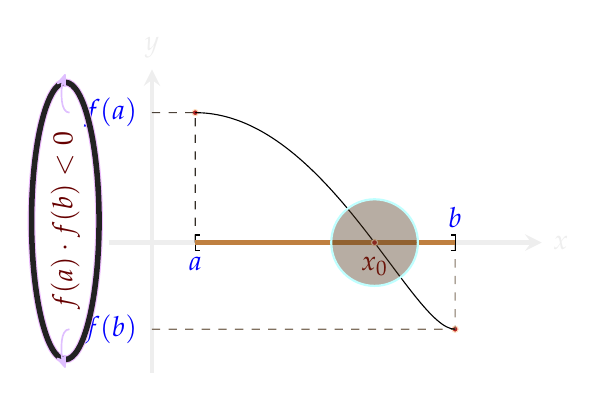
\begin{tikzpicture}[scale =0.55]
				\coordinate (A) at (-1, 3);
				\coordinate (B) at (5, -2);
				\coordinate (O) at (-2, 0);
				
				\draw[draw=w, ultra thick, -stealth] (-3, 0) -- (7, 0) node[text=w, right] {$x$};
				\draw[draw=w, ultra thick, -stealth] (-2, -3) -- (-2, 4) node[text=w, above] {$y$};		
			
				\filldraw[draw=o1, fill=firebrick] (A) circle (2pt);
				\filldraw[draw=o1, fill=firebrick] (B) circle (2pt);	
			
				\coordinate (Ax) at (A |- O);
				\coordinate (Ay) at (A -| O);
				
				\coordinate (Bx) at (B |- O);
				\coordinate (By) at (B -| O);
				
				\draw[dashed, draw=o1!20!black] (Ax) -- (A);
				\draw[dashed, draw=o1!30!black] (Ay) -- (A);
				\node[left, outer sep=2pt, text=blue] (ay) at (Ay) {$f(a)$};
				\node[below, outer sep=2pt, text=blue] at (Ax) {$a$};
				
				\draw[dashed, draw=o1!50!black] (Bx) -- (B);
				\draw[dashed, draw=o1!50!black] (By) -- (B);
				\node[left, outer sep=2pt, text=blue] (by) at (By) {$f(b)$};
				\node[above, outer sep=2pt, text=blue] at (Bx) {$b$};
				
				\draw[thin, draw=black] ($(Ax) + (3pt, -5pt)$) -- ++(180:3pt) -- ++(90:10pt) -- ++ (0:3pt);
				\draw[thin, draw=black] ($(Bx) + (-3pt, -5pt)$) -- ++(0:3pt) -- ++(90:10pt) -- ++ (180:3pt);				
				\draw[ultra thick, draw=brown] (Ax) -- (Bx);
				
				\draw[] (A) .. controls +(0:3cm) and +(left:1cm) .. (B); 
				\coordinate (X) at ($(Ax)!.69!(Bx)$);
				\filldraw[draw=o1, fill=firebrick] (X) circle (2pt);
				\node[below, outer sep=2pt, text=red!50!black] at (X) {$x_0$};
						
				\coordinate (F) at ($(Ay)!0.5!(By) + (-2, 0)$);
				\node[shape=ellipse, double=b, double distance=2pt, draw=v2, rotate=90, text=red!40!black, outer sep=3pt] (ff) at (F) {$f(a)\cdot f(b) < 0$};				
				\draw[->, draw=v1, >={Stealth[round]},semithick] (ay) to[out=180, in=90] (ff.east);
				\draw[->, draw=v1, >={Stealth[round]},semithick] (by) to[out=180, in=270] (ff.west);	
				
				\filldraw[draw=b3, thick, fill=brown!40!black, fill opacity=0.4] (X) circle (1cm);
			\end{tikzpicture}
			
		\end{tcolorbox}			
	
	\quad Fie acum $x_1', x_2'$ două rădăcini cosecutive ale derivatei.
	
	\tikz \draw [draw=o1,ultra thick, dashed]
    ($(current page.center)-(0.495\linewidth,0)$) -- 
    ($(current page.center)+(0.495\linewidth,0)$)
    node [midway, fill=b] {\ssmall\textbf{$\color{firebrick} f(x_1')\cdot f(x_2') < 0$ (funcția schimbă semnul)}};
	
	Atunci există o unică rădăcină a funcției în intervalul $(x_1', x_2')$ conform proprietății funcțiilor continue de mai sus.
	
	\tikz \draw [draw=o1,ultra thick, dashed]
    ($(current page.center)-(0.495\linewidth,0)$) -- 
    ($(current page.center)+(0.495\linewidth,0)$)
    node [midway, fill=b, align=center] {\ssmall\textbf{$\color{firebrick} f(x_1')\cdot f(x_2') > 0$} \\  \ssmall\textbf{(funcția are același semn în capetele intervalului)}};
	
\quad Presupunem prin absurd că există un punct $x_0\in\left(x_1', x_2'\right)$ astfel încât $\text{sgn}\left(f(x_0)\right) = -\text{sgn}\left(f(x_1')\right)$ (i.e. un punct în care funcția schimbă semnul față de capetele intervaului). Atunci avem $f(x_1')\cdot f(x_0) < 0 $ și $f(x_0)\cdot f(x_2') < 0 \Rightarrow x_1 \in \left(x_1', x_0\right) \text{ și } x_2 \in\left(x_0, x_2'\right)$ astfel încât $f(x_1) = 0$ și $f(x_2) = 0$. Dar astfel obținem o contradicție cu faptul că între două rădăcini consecutive ale derivatei există cel mult o rădăcină a funcției. Deci dacă funcția nu schimbă semnul în capetele intervalului, atunci nu schimbă semnul nici în interiorul intervalului. Momentan știm că funcția nu schimbă semnul, dar mai trebuie să stabilim dacă poate să fie $0$.\\

\quad Presupunem acum prin absurd că există un $x_0\in\left(x_1', x_2'\right)$ astfel încât $f(x_0) = 0$. Dar, cum în restul punctelor funcția are același semn sau e egală cu zero, atunci în $x_0$ avem un punct de extrem local, și în plus este în interiorul intervalului, deci conform \textit{teoremei lui Fermat}: $f'(x_0) = 0.$ Obținem o contradicție cu faptul că $x_1', x_2'$ sunt rădăcini consecutive ale derivatei (nu poate să mai existe un alt punct $x_0$ pentru care $f'(x_0) = 0$).\\

\quad În concluzie avem:
	
	\begin{quotebox}[brown]
	 \quad Considerăm $f:\left[a, b\right]\to\mathbb{R}$ o funcție care respectă condițiile \textit{teoremei lui Rolle} și $x_1', x_2'\in\left(a, b\right)$ rădăcini consecutive ale derivatei. Atunci:
	 \begin{itemize}
	 \color{firebrick}
	 \item dacă $f(x_1')\cdot f(x_2') < 0 \Rightarrow \text{\color{v1!70!black} există unic } x_0 \in \left(x_1', x_2'\right) \text{ a.î. } f(x_0) = 0$ \\
	 \item dacă $f(x_1')\cdot f(x_2') > 0 \Rightarrow \text{\color{v1!70!black} nu există } x_0 \in \left(x_1', x_2'\right) \text{ a.î. } f(x_0) = 0$ \\
	 \item dacă $f(x_1') = 0 \Rightarrow  x_1' \text{\color{v1!70!black} este rădăcină multiplă } \text{(la fel pentru } x_2')$
	 \end{itemize}
	 \end{quotebox}
	\end{conceptbox}
\end{multicols*}
\newpage

\begin{multicols*}{2}
	\begin{conceptbox}[yellow!80!black!60!red]{ȘIRUL LUI ROLLE}
		\nc[o1!70!black]{CONSTRUCȚIE}
		
		\quad Fie $I\subseteq \mathbb{R}$ \textbf{\textit{\textcolor{firebrick}{un interval}}} și fie $f:I\to\mathbb{R}$  o funcție continuă pe $I$ și derivabilă pe interiorul intervalului $I$. Considerăm în continuare $x_1<x_2<x_3<\dots < x_{n-1} < x_n$ rădăcinile derivatei ordonate crescător (deci consecutive). \textbf{\textcolor{firebrick}{\textit{Șirul lui Rolle}}} este șirul alcătuit din \textbf{\textcolor{firebrick}{\textit{semnele valorilor}}} funcției $f$ în zerourile derivatei: $\displaystyle\left(f(x_i)\right)_{i=\overline{1, n}}$. Mai exact:
		\begin{quotebox}[gray]
		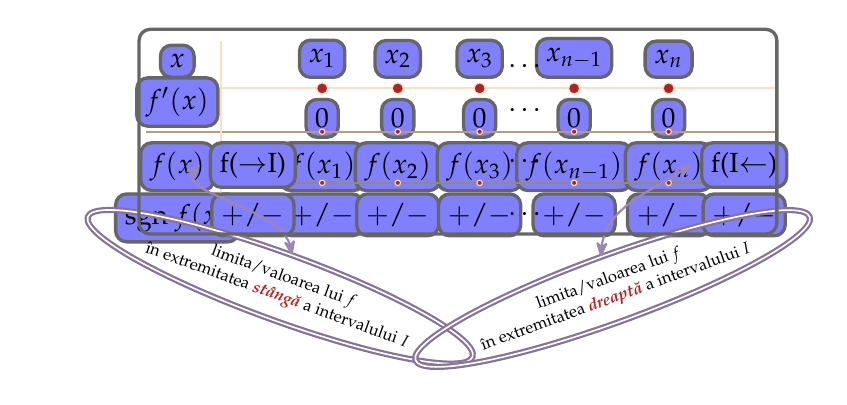
\begin{tikzpicture}[trim left=-5.5cm]
			\coordinate (A1) at (-4, 0);
			\coordinate (A2) at (4, 0);
			
			\draw[draw=o1, thick] (A1) -- (A2);			
			
			\foreach \i/\p in {1/.28, 2/.4, 3/.53, 4/.68, 5/.83}{
				\coordinate (A1\i) at ($(A1)!\p!(A2)$);			
			};
			\foreach \i/\x in {1/1, 2/2, 3/3, 4/n-1, 5/n}{
				\node[shape=rectangle, draw=black!60, fill=blue!50, rounded corners, very thick ,above, outer sep=4pt] at (A1\i) {$x_{\x}$};	
				\node[shape=rectangle, draw=black!60, fill=blue!50, rounded corners, very thick ,below, outer sep=4pt] at (A1\i) {$0$};	
			};
			\foreach \i/\p in {1/.3, 2/.4, 3/.5, 4/.8, 5/.9}{
				\filldraw[draw=o1, fill=firebrick] (A1\i) circle (2pt);		
			};
			
			\coordinate (B1) at ($(A1) + (down:5.5mm)$);
			\coordinate (B2) at ($(A2) + (down:5.5mm)$);
			\draw[draw=o1!70!black, thick] (B1) -- (B2);	
			
			\foreach \i/\p in {1/.28, 2/.4, 3/.53, 4/.68, 5/.83}{
				\coordinate (B1\i) at ($(B1)!\p!(B2)$);			
			};	
			\foreach \i/\p in {1/.3, 2/.42, 3/.5, 4/.8, 5/.9}{
				\filldraw[draw=o1, fill=firebrick] (B1\i) circle (1pt);		
			};	
			\foreach \i/\x in {1/1, 2/2, 3/3, 4/n-1, 5/n}{	
				\node[shape=rectangle, draw=black!60, fill=blue!50, rounded corners, very thick ,below, outer sep=4pt] at (B1\i) {$f(x_{\x})$};};	
				
			\coordinate (C1) at ($(B1) + (down:6.5mm)$);
			\coordinate (C2) at ($(B2) + (down:6.5mm)$);
			\draw[draw=o1!60!black, thick] (C1) -- (C2);	
			
			\foreach \i/\p in {1/.28, 2/.4, 3/.53, 4/.68, 5/.83}{
				\coordinate (C1\i) at ($(C1)!\p!(C2)$);			
			};	
			\foreach \i/\p in {1/.3, 2/.4, 3/.5, 4/.8, 5/.9}{
				\filldraw[draw=o1, fill=firebrick] (C1\i) circle (1pt);		
			};	
			
			\foreach \i in {1, 2, 3, 4, 5}{	
				\node[shape=rectangle, draw=black!60, fill=blue!50, rounded corners, very thick ,below, outer sep=4pt] at (C1\i) {$+/-$};
			};
			
			\foreach \L in {A, B, C}{
					\coordinate (\L10) at ($(\L1)!0.05!(\L2)$);	
			};
			
			\node[shape=rectangle, draw=black!60, fill=blue!50, rounded corners, very thick ,above, outer sep=4pt, minimum width=4mm] at (A10) {$x$};
			\node[shape=rectangle, draw=black!60, fill=blue!50, rounded corners, very thick ,above, outer sep=2pt] at (B10) {$f'(x)$};
			\node[shape=rectangle, draw=black!60, fill=blue!50, rounded corners, very thick ,below, outer sep=4pt] at (B10) {$f(x)$};
			\node[shape=rectangle, draw=black!60, fill=blue!50, rounded corners, very thick ,below, outer sep=4pt] at (C10) {$\text{sgn }f(x)$}; 
			
			\coordinate (A01) at ($(A1)!0.12!(A2) + (up:6mm)$);		
			\coordinate (C01) at ($(C1)!0.12!(C2) + (down:6mm)$);
			\draw[o1, thick] (A01) -- (C01);
			
			
			\foreach \i in {A, B, C}{
					\coordinate (\i101) at ($(\i13)!.5!(\i14)$);	
					\node[above, outer sep = 4pt] at (\i101) {$\dots$};	
			};
			
			\node[] at ($(C13)!.5!(C14) + (down:4mm)$) {$\dots$};	
			
			\coordinate (Bl1) at ($(B1)!.17!(B2)$);
			\coordinate (Bl2) at ($(B1)!.95!(B2)$);
			\coordinate (Cl1) at ($(C1)!.17!(C2)$);
			\coordinate (Cl2) at ($(C1)!.95!(C2)$);				
			
			
			\node[shape=rectangle, draw=black!60, fill=blue!50, rounded corners, very thick ,below, outer sep=4pt] at (Cl1) {$+/-$};
			\node[shape=rectangle, draw=black!60, fill=blue!50, rounded corners, very thick ,below, outer sep=4pt] at (Cl2) {$+/-$};	
			\node[shape=rectangle, draw=black!60, fill=blue!50, rounded corners, very thick ,below, outer sep=4pt] (FS) at (Bl1) {f($\rightarrow$I)};
			\node[shape=rectangle, draw=black!60, fill=blue!50, rounded corners, very thick ,below, outer sep=4pt] (FD) at (Bl2) {f(I$\leftarrow$)};		
			
			\node[shape=ellipse, draw=v1!60!black, double, thick, rotate=-20, align=center, scale=0.6] (FSE) at ($(Bl1) + (-80:2cm)$) {limita/valoarea lui $f$ \\ în extremitatea \textbf{\textcolor{firebrick}{\textit{stângă}}} a intervalului $I$};
			
			\draw[<->, draw=v1!70!black, >={Stealth[round]},thick] (FS.west) to[out=-145, in=90] (FSE.north);		
			
			\node[shape=ellipse, draw=v1!60!black, double, thick, rotate=20, align=center, scale=0.6] (FDE) at ($(Bl2) + (-130:2.6cm)$) {limita/valoarea lui $f$ \\ în extremitatea \textbf{\textcolor{firebrick}{\textit{dreaptă}}} a intervalului $I$};
			
			\draw[<->, draw=v1!70!black, >={Stealth[round]},thick] (FD.west) to[out=-145, in=90] (FDE.north);			
			
			\node[shape=rectangle, draw=black!60, rounded corners, very thick, outer sep=2pt, minimum width=8.1cm, minimum height=2.6cm] at ($(B1)!.5!(B2) + (left:1pt)$) {};
			
			
		\end{tikzpicture}		
		\end{quotebox}
		\nc[o1]{REGULI}
		
		\quad Dacă în \textit{șirul lui Rolle} avem:
		\begin{itemize}
			\item \textbf{\textit{\textcolor{firebrick}{schimbare de semn}}} atunci există o unică rădăcină a funcției în acel interval\\
			\item \textbf{\textit{\textcolor{firebrick}{același semn}}} atunci nu există rădăcini ale funcției în acel interval\\
			\item \textbf{\textit{\textcolor{firebrick}{0}}} atunci acea rădăcină a derivatei este de fapt rădăcină multiplă a funcției
		\end{itemize}
		
	\quad Primul și ultimul semn se compară cu semnul valorii/limitei funcției în extremitățile intervalului.
	\end{conceptbox}	
	\begin{conceptbox}[blue!60!yellow]{Exemplul 1}
	\quad Fie $f:\mathbb{R}\to\mathbb{R}, f(x) =\dfrac{1}{16}\left( x^4 - 8x^3 + 16x^2 - 16\right)$. $f$ e continuă și derivabilă pe $\mathbb{R}$.\\
	
	$f'(x) =\dfrac{1}{16}\left( 4x^3 - 24x^2 + 32x\right) = \dfrac{x}{4}\left(x^2 - 6x + 8\right)= \dfrac{x}{4}\left(x-2\right)\left(x-4\right)$\\
	$f'(x) = 0 \Leftrightarrow \dfrac{x}{4}(x-2)(x-4) = 0 \Leftrightarrow x \in \{0, 2, 4\}$\\
	$f(0) = -1; f(2) = 0; f(4) = -1; \displaystyle\lim_{x\to -\infty} f(x) = \lim_{x\to+\infty} f(x) = +\infty$\\
	\begin{center}
	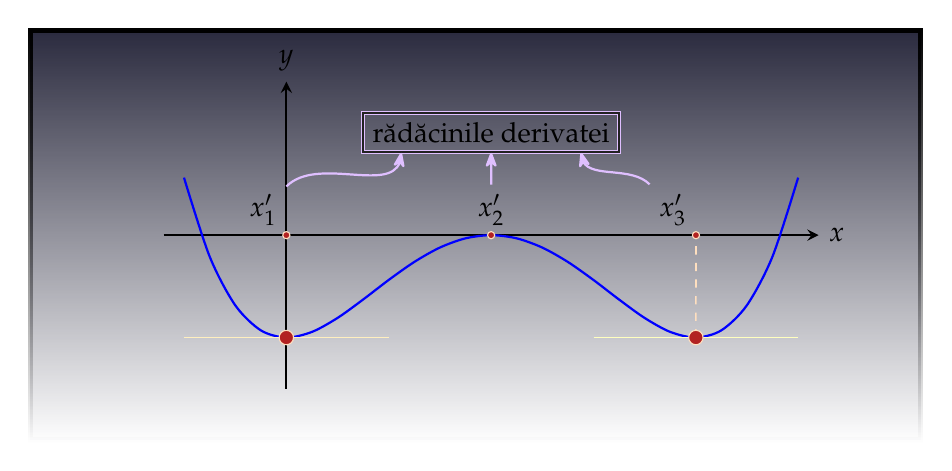
\begin{tikzpicture}[scale=1.3]
		\filldraw[line width = 2pt, path fading=south, fill=blue!60!yellow!40!black] (-2.5, -2) rectangle (6.2, 2);
		\draw[thick, -stealth] (-1.2, 0) -- (5.2, 0) node[right] {$x$};
		\draw[thick, -stealth] (0, -1.5) -- (0, 1.5) node[above] {$y$};
	
		\draw[domain=-1:5, thick, smooth, variable=\x, blue] plot ({\x}, {\x*\x*\x*\x/16 - \x*\x*\x/2 + \x*\x - 1});
		
		\coordinate (O) at (0, 0);
		\coordinate (D1) at (0, -1);
		\coordinate (D2) at (2, 0);
		\coordinate (D3) at (4, -1);
		
		\draw[y3, semithick] ($(D1) + (left:1cm)$) -- ($(D1) + (right:1cm)$);
		\draw[y1, semithick] ($(D3) + (left:1cm)$) -- ($(D3) + (right:1cm)$);
		
		\filldraw[draw=o1, fill=firebrick] (D1) circle (2pt);
		\coordinate (D1x) at (D1 |- O);
		\coordinate (D1y) at (D1 -| O);
		\node[above left] (d1) at (D1x) {$x_1'$}; 
		\filldraw[draw=o1, fill=firebrick] (D1x) circle (1pt);
		
		\filldraw[draw=o1, fill=firebrick] (D2) circle (1pt);
		\coordinate (D2x) at (D2 |- O);
		\coordinate (D2y) at (D2 -| O);
		\node[above] (d2) at (D2x) {$x_2'$}; 
%		\filldraw[draw=o1, fill=firebrick] (D2x) circle (1pt);
		
		
		\coordinate (D3x) at (D3 |- O);
		\coordinate (D3y) at (D3 -| O);
		\node[above left] (d3) at (D3x) {$x_3'$}; 
		\draw[draw=o1, semithick, dashed] (D3) -- (D3x);		
		\filldraw[draw=o1, fill=firebrick] (D3) circle (2pt);		
		\filldraw[draw=o1, fill=firebrick] (D3x) circle (1pt);	
		
		
		\node[double=b, draw=v1] (RD) at ($(D2) + (up:1cm)$) {rădăcinile derivatei};
		\draw[->, draw=v1, >={Stealth[round]},thick] (d1) to[in=-90] ($(RD.south west)!.3!(RD.south)$);
		\draw[->, draw=v1, >={Stealth[round]},thick] (d2) to[] (RD.south);
		\draw[->, draw=v1, >={Stealth[round]},thick] (d3.north west) to[out=135, in=-90] ($(RD.south east)!.3!(RD.south)$);
	
	\end{tikzpicture}
		
	\begin{tblr}{colspec={c|ccccc},
		hline{2} = {2pt, solid},
		hline{3-4} = {.5pt, solid},
	}
		x & $-\infty$ & 0 & 2 & 4 & $+\infty$ \\
		f'(x) & & 0 & 0 & 0 & \\ 
		f(x) & $+\infty$ & -1 & 0 & -1 & $+\infty$\\
		sgn f(x) & + & - & 0 & - & +\\
	\end{tblr}
		
	\end{center}
	
	Avem:
	\begin{itemize}
		\item schimbare de semn $-\infty\to 0 \Rightarrow \exists!\; x_1 \in \left(-\infty, 0\right) \text{ a.î. } f(x_1) = 0$\\
		\item $f(2) = f'(2) = 0 \Rightarrow x_2 = 2 \to $ rădăcină multiplă\\
		\item schimbare de semn $4\to +\infty \Rightarrow \exists!\; x_3 \in \left(4, +\infty \right) \text{ a.î. } f(x_3) = 0$\\
	\end{itemize}
Având o funcție polinomială de ordin 4, știm că $x_2=2$ este rădăcină multiplă de ordin 2.
	\end{conceptbox}
	\begin{conceptbox}[b3!40!yellow]{EXEMPLUl 2}
	
	\quad Fie $f:\mathbb{R}_{\setminus\{-1, 1\}}\to\mathbb{R}, f(x) := \dfrac{1}{8}\cdot\dfrac{x^3}{x^2 - 1} + \dfrac{1}{2}$. Să se determine intervalele de separare a rădăcinilor funcției $f$.
	\begin{center}
		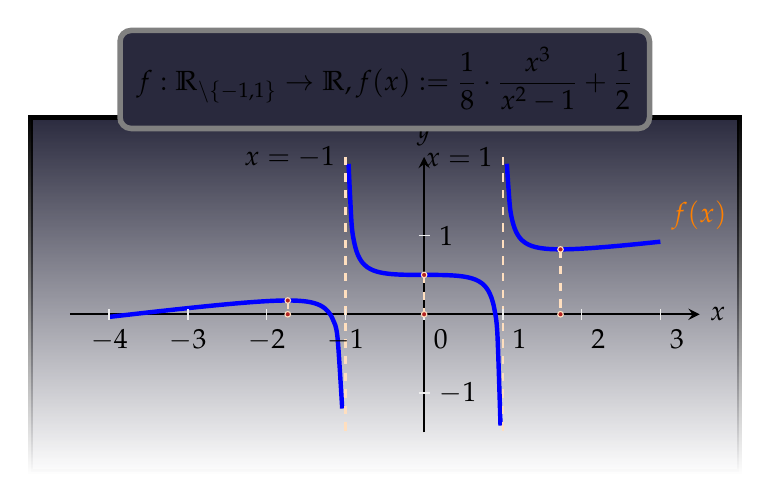
\begin{tikzpicture}
			\filldraw[line width = 2pt, path fading=south, fill=blue!60!yellow!40!black] (-5, -2) rectangle (4, 2.5);
		\draw[thick, -stealth] (-4.5, 0) -- (3.5, 0) node[right] {$x$};
		\draw[thick, -stealth] (0, -1.5) -- (0, 2) node[above] {$y$};
		
		\draw[domain=-4:-1.04, ultra thick, smooth, variable=\x, blue, samples=50] plot ({\x}, {1/8 * (\x*\x*\x)/(\x*\x-1) + .5});
		\draw[domain=-0.96:0.97, ultra thick, smooth, variable=\x, blue, samples=50] plot ({\x}, {1/8 * (\x*\x*\x)/(\x*\x-1) + .5});
		\draw[domain=1.05:3, ultra thick, smooth, variable=\x, blue, samples=50] plot ({\x}, {1/8 * (\x*\x*\x)/(\x*\x-1) + .5}) node[above right, text=orange] {$f(x)$};
		
%		\draw[domain=-1.6:0.3, thick, smooth, variable=\x, red, samples=50] plot ({\x}, {(2*\x*\x*\x - 2*\x)/(2*\x - 1)}) node[below left, text=orange] {$f'(x)$};
%		\draw[domain=0.75:1.4, thick, smooth, variable=\x, red, samples=50] plot ({\x}, {(2*\x*\x*\x - 2*\x)/(2*\x - 1 )});
		
%		\draw[draw=o1, fill=firebrick] (1, -3) circle (1pt);
		\draw[dashed, draw=o1, thick] ($(-1, 0) + (up:2cm)$) node[left] {$x = -1$} -- ($(-1, 0) + (down:1.5cm)$);
		\draw[dashed, draw=o1, thick] ($(1, 0) + (up:2cm)$) node[left] {$x = 1$} -- ($(1, 0) + (down:1.5cm)$);
		
		
		\foreach \i in {-4, -3, -2, -1}{
			\coordinate (p) at (\i, 0);
			\coordinate (pd) at ($(p) + (down:2pt)$);
			\coordinate (pu) at ($(p) + (up:2pt)$);
			
			\draw[draw=w, semithick] (pd) -- (pu);
			\node[below] at (pd) {$\i$};
		};		
		\foreach \i in {0, 1, 2, 3}{
			\coordinate (p) at (\i, 0);
			\coordinate (pd) at ($(p) + (down:2pt)$);
			\coordinate (pu) at ($(p) + (up:2pt)$);
			
			\draw[draw=w, semithick] (pd) -- (pu);
			\node[below right] at (pd) {$\i$};
		};
		\foreach \i in {-1, 1}{
			\coordinate (p) at (0, \i);
			\coordinate (pr) at ($(p) + (right:2pt)$);
			\coordinate (pl) at ($(p) + (left:2pt)$);
			
			\draw[draw=w, semithick] (pl) -- (pr);
			\node[right] at (pr) {$\i$};
		};	
		
		\coordinate (d1) at (-1.732, 0.175);
		\coordinate (d2) at (0, 0.5);
		\coordinate (d3) at (1.732, 0.824);	
		
		\foreach \i in {1, 2, 3}{
			\coordinate (xd\i) at (d\i |- 0, 0);
			
			\draw[draw=o1, dashed, thick] (d\i) -- (xd\i);
			\filldraw[draw=o1, fill=firebrick] (xd\i) circle (1pt);
			\filldraw[draw=o1, fill=firebrick] (d\i) circle (1pt);	
		};
		
		\node[shape=rectangle, line width=2pt, rounded corners, draw=gray, fill = blue!60!yellow!40!black, above=-5pt, inner sep=6pt] at (-0.5, 2.5)	{$f:\mathbb{R}_{\setminus\{-1, 1\}}\to\mathbb{R}, f(x) := \dfrac{1}{8}\cdot\dfrac{x^3}{x^2 - 1} + \dfrac{1}{2}$};
		\end{tikzpicture}
	\end{center}
	f este continuă și derivabilă pe $\mathbb{R}_{\setminus \{\pm 1\}}$ și $f'(x) = \dfrac{1}{8}\cdot\dfrac{x^2(x^2-3)}{(x^2 - 1)^2} (\forall)\; x\in\mathbb{R}_{\setminus \{\pm 1\}}$.\\
	$f'(x) = 0 \Leftrightarrow x\in\{-\sqrt{3}, 0, \sqrt{3}\}$ și: $f(-\sqrt{3}) = \dfrac{8-3\sqrt{3}}{16}>0;f(0) = \dfrac{1}{2}; f(\sqrt{3}) = \dfrac{8+3\sqrt{3}}{16} > 0;\displaystyle\lim_{x\to -\infty} = -\infty;\lim_{x\to+\infty} = +\infty$\\
	$\displaystyle\lim_{x\nearrow -1}f(x) = -\infty; \lim_{x\searrow -1} f(x) = +\infty;\lim_{x\nearrow 1}f(x) = -\infty; \lim_{x\searrow 1} f(x) = +\infty;$
	
	\begin{center}
	\begin{tblr}{colspec={c|ccccccc},
		hline{2} = {2pt, solid},
		hline{3-4} = {.5pt, solid},
	}
		x & $-\infty$ & $-\sqrt{3}$ & -1 & 0 & 1 & $\sqrt{3}$ & $+\infty$ \\
		f'(x) & & 0 & $\Big|$ & 0 & $\Big|$ & 0 & & \\ 
		f(x) & $-\infty$ & $\dfrac{8-3\sqrt{3}}{16}$ & $\prescript{}{-\infty}{\Big|^{+\infty}}$ & $\dfrac{1}{2}$ & $\prescript{}{-\infty}{\Big|^{+\infty}}$ & $\dfrac{8+3\sqrt{3}}{16}$ & $+\infty$\\
		sgn f(x) & - & + & $-\Big| +$ & + & $-\Big| +$ & + & +\\
	\end{tblr}
	\end{center}
	Deci avem:
	\begin{itemize}
		\item $\exists!\; x_1\in\left(-\infty, -\sqrt{3}\right)$ a.î. $f(x_1) = 0$
		\item $\exists!\; x_2\in\left(-\sqrt{3}, -1\right)$ a.î. $f(x_2) = 0$
		\item $\exists!\; x_3\in\left(0, 1\right)$ a.î. $f(x_3) = 0$
		
	\end{itemize}
	\end{conceptbox}
	\begin{conceptbox}[purple!70!green]{EXEMPLUL 3}
	
	\quad Discutați numărul rădăcinilor funcției $f:\mathbb{R}\to\mathbb{R}, f(x) = 2x^3 - 15x^2+36x - 6+m, m\in\mathbb{R}$ în raport cu valorile parametrului $m$.\\
	
	$f'(x) = 6x^2 - 30x + 36\\ f'(x) = 0 \Leftrightarrow 6x^2 - 30x + 36 = 0 \Leftrightarrow x^2 - 5x + 6 = 0\Leftrightarrow x\in\{2, 3\}$\\
	$f(2) = m+22; f(3) = m+21;\displaystyle\lim_{x\to-\infty} f(x) = -\infty;\lim_{x\to+\infty} f(x) = + \infty$\\
	
	\begin{center}
	\begin{tblr}{colspec={Q[c,m]|Q[c,m]Q[c,m]Q[c,m]Q[c,m]|Q[c,m]|},
		hline{1, 9} = {}{6}{.5pt, solid},
		hline{2} = {2pt, solid},
		hline{3-8} = {.5pt, solid},
		cell{1}{6} = {r=3, c=1}{c},
	}
		x & $-\infty$ & 2 & 3 & $+\infty$ & {Separarea \\ soluțiilor}\\
		f'(x) & & 0 & 0 & &\\ 
		f(x) & $-\infty$ & $m+22$ & $m+21$ & $+\infty$ & \\
		$m\in \left(-\infty, -22\right)$ & - & - & - & + & $x_1\in\left(-\infty, 2\right)$ \\
		$m = -22$ & - & 0 & - & + & {$x_1 = 2$-rădăcină multiplă \\ $x_2\in\left(3, +\infty\right)$} \\
		$m\in \left(-22, -21\right)$ & - & + & - & + & {$x_1\in\left(-\infty, 2\right)$ \\ $x_2\in\left(2, 3\right)$ \\ $x_3\in\left(3, +\infty\right)$} \\
		$m = -21$ & - & + & 0 & + & {$x_1\in\left(-\infty, 2\right)$ \\ $x_2 = 3$-rădăcină multiplă} \\
		$m\in \left(-21, +\infty\right)$ & - & + & + & + & $x_1\in\left(-\infty, 2\right)$ \\
		
	\end{tblr}
	\end{center}	
	\hfill
	\end{conceptbox}
\end{multicols*}

\end{document}